
\documentclass[spanish,openright]{book}

\usepackage[utf8]{inputenc}
\usepackage[english]{babel}
\usepackage{graphicx}
\usepackage[nottoc]{tocbibind} % para que muestre el apartado de referencias en el índice
\usepackage{lipsum} % Para meter texto random
%%%%%%%%%%%%%%%%%%%%%%%%%%%%%%%
% CONFIGURACIÓN CÓDIGO PYTHON %
%%%%%%%%%%%%%%%%%%%%%%%%%%%%%%%

% Estilo del codigo escrito en el documento

\definecolor{maroon}{cmyk}{0, 0.87, 0.68, 0.32}
\definecolor{halfgray}{gray}{0.55}
\definecolor{ipython_frame}{RGB}{207, 207, 207}
\definecolor{ipython_bg}{RGB}{247, 247, 247}
\definecolor{ipython_red}{RGB}{186, 33, 33}
\definecolor{ipython_green}{RGB}{0, 128, 0}
\definecolor{ipython_cyan}{RGB}{64, 128, 128}
\definecolor{ipython_purple}{RGB}{170, 34, 255}

\usepackage{listings}
\lstset{
    breaklines=true,
    xleftmargin=.29in,
    xrightmargin=.29in,
    extendedchars=true,
    literate=
    {á}{{\'a}}1 {é}{{\'e}}1 {í}{{\'i}}1 {ó}{{\'o}}1 {ú}{{\'u}}1
    {Á}{{\'A}}1 {É}{{\'E}}1 {Í}{{\'I}}1 {Ó}{{\'O}}1 {Ú}{{\'U}}1
    {à}{{\`a}}1 {è}{{\`e}}1 {ì}{{\`i}}1 {ò}{{\`o}}1 {ù}{{\`u}}1
    {À}{{\`A}}1 {È}{{\'E}}1 {Ì}{{\`I}}1 {Ò}{{\`O}}1 {Ù}{{\`U}}1
    {ä}{{\"a}}1 {ë}{{\"e}}1 {ï}{{\"i}}1 {ö}{{\"o}}1 {ü}{{\"u}}1
    {Ä}{{\"A}}1 {Ë}{{\"E}}1 {Ï}{{\"I}}1 {Ö}{{\"O}}1 {Ü}{{\"U}}1
    {â}{{\^a}}1 {ê}{{\^e}}1 {î}{{\^i}}1 {ô}{{\^o}}1 {û}{{\^u}}1
    {Â}{{\^A}}1 {Ê}{{\^E}}1 {Î}{{\^I}}1 {Ô}{{\^O}}1 {Û}{{\^U}}1
    {œ}{{\oe}}1 {Œ}{{\OE}}1 {æ}{{\ae}}1 {Æ}{{\AE}}1 {ß}{{\ss}}1
    {ç}{{\c c}}1 {Ç}{{\c C}}1 {ø}{{\o}}1 {å}{{\r a}}1 {Å}{{\r A}}1
    {€}{{\EUR}}1 {£}{{\pounds}}1
}

%%
%% Python definition (c) 1998 Michael Weber
%% Additional definitions (2013) Alexis Dimitriadis
%% modified by me (should not have empty lines)
%%
\lstdefinelanguage{iPython}{
    morekeywords={access,and,break,class,continue,def,del,elif,else,except,exec,finally,for,from,global,if,import,in,is,lambda,not,or,pass,print,raise,return,try,while},%
    %
    % Built-ins
    morekeywords=[2]{abs,all,any,basestring,bin,bool,bytearray,callable,chr,classmethod,cmp,compile,complex,delattr,dict,dir,divmod,enumerate,eval,execfile,file,filter,float,format,frozenset,getattr,globals,hasattr,hash,help,hex,id,input,int,isinstance,issubclass,iter,len,list,locals,long,map,max,memoryview,min,next,object,oct,open,ord,pow,property,range,raw_input,reduce,reload,repr,reversed,round,set,setattr,slice,sorted,staticmethod,str,sum,super,tuple,type,unichr,unicode,vars,xrange,zip,apply,buffer,coerce,intern},%
    %
    sensitive=true,%
    morecomment=[l]\#,%
    morestring=[b]',%
    morestring=[b]",%
    %
    morestring=[s]{'''}{'''},% used for documentation text (mulitiline strings)
    morestring=[s]{"""}{"""},% added by Philipp Matthias Hahn
    %
    morestring=[s]{r'}{'},% `raw' strings
    morestring=[s]{r"}{"},%
    morestring=[s]{r'''}{'''},%
    morestring=[s]{r"""}{"""},%
    morestring=[s]{u'}{'},% unicode strings
    morestring=[s]{u"}{"},%
    morestring=[s]{u'''}{'''},%
    morestring=[s]{u"""}{"""},%
    %
    % {replace}{replacement}{lenght of replace}
    % *{-}{-}{1} will not replace in comments and so on
    literate=
    {á}{{\'a}}1 {é}{{\'e}}1 {í}{{\'i}}1 {ó}{{\'o}}1 {ú}{{\'u}}1
    {Á}{{\'A}}1 {É}{{\'E}}1 {Í}{{\'I}}1 {Ó}{{\'O}}1 {Ú}{{\'U}}1
    {à}{{\`a}}1 {è}{{\`e}}1 {ì}{{\`i}}1 {ò}{{\`o}}1 {ù}{{\`u}}1
    {À}{{\`A}}1 {È}{{\'E}}1 {Ì}{{\`I}}1 {Ò}{{\`O}}1 {Ù}{{\`U}}1
    {ä}{{\"a}}1 {ë}{{\"e}}1 {ï}{{\"i}}1 {ö}{{\"o}}1 {ü}{{\"u}}1
    {Ä}{{\"A}}1 {Ë}{{\"E}}1 {Ï}{{\"I}}1 {Ö}{{\"O}}1 {Ü}{{\"U}}1
    {â}{{\^a}}1 {ê}{{\^e}}1 {î}{{\^i}}1 {ô}{{\^o}}1 {û}{{\^u}}1
    {Â}{{\^A}}1 {Ê}{{\^E}}1 {Î}{{\^I}}1 {Ô}{{\^O}}1 {Û}{{\^U}}1
    {œ}{{\oe}}1 {Œ}{{\OE}}1 {æ}{{\ae}}1 {Æ}{{\AE}}1 {ß}{{\ss}}1
    {ç}{{\c c}}1 {Ç}{{\c C}}1 {ø}{{\o}}1 {å}{{\r a}}1 {Å}{{\r A}}1
    {€}{{\EUR}}1 {£}{{\pounds}}1,
    %
    literate=
    *{+}{{{\color{ipython_purple}+}}}1
    {-}{{{\color{ipython_purple}-}}}1
    {*}{{{\color{ipython_purple}$^\ast$}}}1
    {/}{{{\color{ipython_purple}/}}}1
    {^}{{{\color{ipython_purple}\^{}}}}1
    {?}{{{\color{ipython_purple}?}}}1
    {!}{{{\color{ipython_purple}!}}}1
    {\%}{{{\color{ipython_purple}\%}}}1
    {<}{{{\color{ipython_purple}<}}}1
    {>}{{{\color{ipython_purple}>}}}1
    {|}{{{\color{ipython_purple}|}}}1
    {\&}{{{\color{ipython_purple}\&}}}1
    {~}{{{\color{ipython_purple}~}}}1
    %
    {==}{{{\color{ipython_purple}==}}}2
    {<=}{{{\color{ipython_purple}<=}}}2
    {>=}{{{\color{ipython_purple}>=}}}2
    %
    {+=}{{{+=}}}2
    {-=}{{{-=}}}2
    {*=}{{{$^\ast$=}}}2
    {/=}{{{/=}}}2,
    %
%   identifierstyle=\color{red}\ttfamily,
    commentstyle=\color{ipython_cyan}\ttfamily,
    stringstyle=\color{ipython_red}\ttfamily,
    keepspaces=true,
    showspaces=false,
    showstringspaces=false,
    %
    rulecolor=\color{ipython_frame},
    frame=single,
    frameround={t}{t}{t}{t},
    framexleftmargin=6mm,
    numbers=left,
    numberstyle=\tiny\color{halfgray},
    %
    %
    backgroundcolor=\color{ipython_bg},
    %   extendedchars=true,
    basicstyle=\scriptsize\ttfamily,
    keywordstyle=\color{ipython_green}\ttfamily,
    escapechar=\¢,escapebegin=\color{ipython_green},
}

\makeglossaries % Genera la base de datos de acrónimos
\newacronym{aboda}{ABODA}{Abandoned Objects Dataset}
\newacronym{doa}{DOA}{Detección de Objetos Abandonados}
\newacronym{ap}{AP}{Average precision}
\newacronym{asff}{ASFF}{Adaptively Spatial Feature Fusion}
\newacronym{auc}{AUC}{Area Under the ROC Curve}
\newacronym{avss}{AVSSAB2007}{Advanced Video and Signal based Surveillance Abandoned Baggage}


\newacronym{bow}{BOW}{Bag of Words}


\newacronym{cnn}{CNN}{Redes Neuronales Convolucionales}
\newacronym{coco}{MS COCO}{Microsoft Common Objects in Context (test-dev 2017)}
\newacronym{cpu}{CPU}{Central Processing Unit}
\newacronym{cuda}{CUDA}{Compute Unified Device Architecture}
\newacronym{cudnn}{cuDNN}{CUDA Deep Neural Network}


\newacronym{deepsort}{DeepSORT}{Simple Online and Realtime Tracking with a Deep Association Metric}
\newacronym{dnn}{DNN}{Deep Neural Network}
\newacronym{dssd}{DSSD}{Deconvolutional Single Shot Detector}


\newacronym{eps}{EPS}{Escuela Politécnica Superior}


\newacronym{fairmot}{FairMOT}{On the Fairness of Detection and Re-Identification in Multiple Object Tracking}
\newacronym{fn}{FN}{False Negative}
\newacronym{fp}{FP}{False Positive}
\newacronym{fc}{FC}{Fully Connected}
\newacronym{flops}{FLOPS}{Floating Point Operations Per Second}
\newacronym{fpn}{FPN}{Feature Pyramid Network}
\newacronym{fps}{FPS}{Frames Per Second}


\newacronym{gba2018}{GBA2018}{GEINTRA Behaviour Analysis 2018}
\newacronym{geintra}{GEINTRA}{Grupo de Ingeniería Electrónica Aplicada a Espacios Inteligentes y Transporte}
\newacronym{gpu}{GPU}{Graphics Processing Unit}


\newacronym{hog}{HOG}{Histograma de Gradientes Orientados}


\newacronym{ide}{IDE}{Integrated Development Environment}
\newacronym{iou}{IoU}{Intersection over Union}
\newacronym{ipm}{IPM}{Inverse Perspective Mapping}


\newacronym{map}{mAP}{Mean average precision}
\newacronym{mlp}{MLP}{Multilayer perceptron}
\newacronym{mot}{MOT}{Multi Object Tracking}


\newacronym{nas}{NAS}{Network Architecture Search}


\newacronym{pan}{PAN}{Path Aggregation Network}
\newacronym{pets}{PETS2007}{Performance Evaluation of Tracking and Surveillance 2007}


\newacronym{oidv4}{OIDv4}{Open Images Dataset v4}


\newacronym{r-cnn}{R-CNN}{Region Based Convolutional Neural Networks}
\newacronym{rgb}{RGB}{Red, Green, Blue}
\newacronym{roi}{ROI}{Region of interest}
\newacronym{rpn}{RPN}{Region Proposal Network}


\newacronym{sfam}{SFAM}{Scale-wise Feature Aggregation Module}
\newacronym{sort}{SORT}{Simple Online and Realtime Tracking}
\newacronym{spp}{SPP}{Spatial Pyramid Pooling}
\newacronym{ssd}{SSD}{Single Shot MultiBox Detector}
\newacronym{svdd}{SVDD}{Support Vector Data Description}
\newacronym{svm}{SVM}{Support Vector Machines}


\newacronym{tfm}{TFM}{Trabajo Fin de Máster}
\newacronym{tn}{TN}{True Negative}
\newacronym{tp}{TP}{True Positive}


\newacronym{uah}{UAH}{Universidad de Alcalá de Henares}


\newacronym{yolo}{YOLO}{You Only Look Once}
\newacronym{yolov4}{YOLOv4}{You Only Look Once v4} % Archivo que contiene la lista de acrónimos

\begin{document}

% Portada

\includepdf[pages={1-3}]{cover/portada.pdf}

% Numeración romana
\frontmatter

% Dedicatoria + agradecimientos
\thispagestyle{empty}

\begin{flushright}

  \topskip0pt
  \vspace*{\fill}

  \textbf{A mi hermano Carlos\ldots}\\

  \vspace{3cm}

  \emph{``Empieza haciendo lo necesario, luego haz lo posible y de
    pronto empezarás a hacer lo imposible.''}\\ Francisco de Asís

\end{flushright}  

\vspace{4cm}
\vspace*{\fill}

\chapter*{Agradecimientos}
\label{cha:agradecimientos}
\markboth{Agradecimientos}{Agradecimientos}

Este trabajo es el fruto de muchas horas de trabajo, tanto de los
autores últimos de los ficheros de la distribución como de todos los que
en mayor o menor medida han participado en él a lo largo de su proceso
de gestación.

Mención especial merece Manuel Ocaña, el autor de la primera versión de
las plantillas de proyectos fin de carrera y tesis doctorales usadas en
el Departamento de Electrónica de la Universidad de Alcalá, con
contribuciones de Jesús Nuevo, Pedro Revenga, Fernando Herránz y Noelia
Hernández.

En la versión actual, la mayor parte de las definiciones de estilos de
partida proceden de la tesis doctoral de Roberto Barra-Chicote, con lo
que gracias muy especiales para él.

También damos las gracias a \dots que nos
han proporcionado secciones completas y ejemplos puntuales de sus
proyectos fin de carrera.

Finalmente, hay incontables contribuyentes a esta plantilla, la mayoría
encontrados gracias a la magia del buscador de Google. Hemos intentado
referenciar los más importantes en los fuentes de la plantilla, aunque
seguro que hemos omitido alguno. Desde aquí les damos las gracias a
todos ellos por compartir su saber con el mundo.

% Resumen/abstract + resumen extendido

\chapter*{Resumen}
\label{cha:resumen}

\addcontentsline{toc}{chapter}{Resumen}

Este Trabajo Fin de Máster tiene como objeto el estudio e implementación de algoritmos empleando redes neuronales convolucionales (\textit{CNN}) con la finalidad de detectar objetos abandonados mediante el uso de aplicaciones de videovigilancia. Estas redes se tratan de algoritmos de aprendizaje supervisado especializados para trabajar con imágenes (poner explicación de DotCSV).

En el presente trabajo se ha realizado un estudio teórico de los distintos algoritmos de detección de objetos sobre determinadas bases de datos así como algoritmos de rastreo o \textit{tracking} disponibles en el Estado del Arte. Para la detección de objetos se ha empleado YOLOv4 \cite{bochkovskiy2020yolov4}. Posteriormente se ha desarrollado un algoritmo de DeepSORT \cite{Wojke2017simple} donde se ha filtrado que rastree únicamente a personas y objetos de interés: mochilas, maletas, bolsos y bolsas de mano. Se ha utilizado COCO \cite{lin2015microsoft} como conjunto de datos ya que se trata de un estándar de referencia muy utilizado en la evaluación del rendimiento de modelos de visión por computador.

Por último se ha implementado y evaluado un algoritmo que determine si un objeto ha sido abandonado o no. Para ello se deberán de tener en cuenta diferentes métricas como el tiempo que el objeto se encuentra estático en un determinado punto o la distancia a la que se encuentra respecto a la persona que lo portaba.

\textbf{Palabras clave:} Redes neuronales convolucionales, YOLOv4, DeepSORT, videovigilancia, visión por computador.

\chapter*{Abstract}
\label{cha:abstract}

\addcontentsline{toc}{chapter}{Abstract}
\noindent
The aim of this Master's Thesis is to study and implement algorithms using convolutional neural networks (\textit{CNN}) in order to detect abandoned objects through the use of video surveillance applications. These networks are specialized supervised learning algorithms for working with images (put DotCSV explanation).

In the present document, has been carried out a theoretical study of the different object detection algorithms on certain databases, as well as tracking algorithms available in the State of the Art. YOLOv4 \cite{bochkovskiy2020yolov4} has been used for object detection. Subsequently, a DeepSORT algorithm \cite{Wojke2017simple} has been developed where it has been filtered that only tracks people and objects of interest: backpacks, suitcases and handbags. COCO \cite{lin2015microsoft} has been used as the dataset as standard benchmark for evaluating the performance of computer vision models.

Finally, an algorithm has been implemented and evaluated to determine whether an object has been abandoned or not. To do this, different metrics must be taken into account, such as the time that the object is static at a certain point or the distance it is from the person who was carrying it.

\textbf{Keywords:} Convolutional Neural Networks, YOLOv4, DeepSORT, Video Surveillance, Computer Vision.

\chapter*{Resumen extendido}
\label{cha:resumen-extendido}

\addcontentsline{toc}{chapter}{Resumen extendido}

La detección de objetos abandonados se trata de una de las aplicaciones más importantes dentro de los sistemas de detección por videovigilancia en los últimos años \cite{DBLP:journals/spm/PlataniotisR05}. La demanda de detección de objetos abandonados esta al alza y se precisa disponer de aplicaciones capaces de detectar y evaluar conductas en tiempo real y con márgenes de error reducidos. Este trabajo pretende cubrir una de las etapas de desarrollo en la detección, la asociación entre persona y objeto, con la finalidad de poder identificar al propietario y determinar si el objeto ha sido abandonado o no.

En este trabajo se realizado un estudio exhaustivo del Estado del Arte actual en estrategias para abordar la problemática de la detección de objetos abandonados mediante el uso de aplicaciones de videovigilancia.

Se ha implementado y evaluado YOLOv4 \cite{bochkovskiy2020yolov4}, un algoritmo de detección de objetos que hace uso de una única red neuronal convolucional para detectar objetos a partir de imágenes. Esta red neuronal, que está previamente entrenada con el dataset de MS COCO \cite{lin2015microsoft}, ha vuelto a ser entrenada con el dataset Open Images Dataset v4 \cite{Kuznetsova_2020} con el objetivo de que solo detecte ciertos objetos de interés: personas, mochilas, bolsos, bolsas de mano, maletines y maletas. Tras el entrenamiento se han calculado las métricas de calidad más utilizadas en la evaluación de algoritmos de detección de objetos para determinar si se superan las del modelo preentrenado del dataset de MS COCO.

El dataset de referencia con el que se obtuvieron mejores métricas en YOLOv4 fue MS COCO. Posteriormente se han realizado evaluaciones sobre los datasets de detección de objetos abandonados PETS2007 \cite{pets2007-dataset}, AVSSAB2007 \cite{AVSSAB2007-dataset}, GBA2018 \cite{gba-dataset} y ABODA \cite{aboda-dataset}. 

En base a YOLOv4 se ha realizado un estudio en el Estado del Arte de los algoritmos de seguimiento más actuales con la finalidad de que asignar una identidad a cada detección. Se ha implementado el algoritmo Deep SORT \cite{Wojke2017simple} junto a YOLOv4. Deep SORT  es un algoritmo predecesor de SORT \cite{Bewley_2016}, que realiza un seguimiento basado en la detección, realizando los procesos de predicción y actualización con filtros de Kalman. Empleando este algoritmo de seguimiento se ha podido rastrear el movimiento de las personas y los objetos asignándoles una identidad única. Del mismo modo que en el algoritmo de detección, se ha evaluado su funcionamiento sobre los datasets más relevantes.

Posteriormente se ha diseño, implementado y evaluado un algoritmo que determine si un objeto ha sido abandonado o no en base a los algoritmos de detección y seguimiento antes nombrados. Para ello, se ha calculado en los 5 primeros segundos del vídeo la distancia existente entre las personas con todos los objetos de interés detectables. Con la distancia mínima que exista entre una persona y un objetos se puede establecer una asociación.

Obtenida la vinculación persona-objeto se puede evaluar el comportamiento calculando la distancia a la que se encuentran en los siguientes fotogramas del vídeo, y así determinar si se produce un abandono del objeto. Otra posibilidad es que el objeto se encuentre durante el transcurso de todo el vídeo estático \cite{luna2018} en el mismo punto y sin asignación con otra persona. En este caso se puede deducir que ese objeto está abandonado sin posibilidad de detectar al propietario.

Con el desarrollo del algoritmo capaz de detectar objetos abandonados se ha evaluado los resultados en distintos escenarios, del mismo modo que con los algoritmo de detección y seguimiento, teniendo como métrica de calidad la tasa de fallos en la determinar si un objeto ha sido abandonado.


% Índices
\hypersetup{linkcolor=\mytoclinkcolor}
\tableofcontents

\hypersetup{linkcolor=\myloflinkcolor}
\listoffigures

\hypersetup{linkcolor=\mylotlinkcolor}
% Para que salga "Índice de tablas" en vez de "Índice de cuadros"
\renewcommand{\listtablename}{Índice de tablas} 
\renewcommand{\tablename}{Tabla}
\listoftables

\hypersetup{linkcolor=\mylollinkcolor}
\renewcommand{\lstlistingname}{Código}
\renewcommand{\lstlistlistingname}{Índice de listados de código fuente}
\lstlistoflistings

% Resto de colores
\hypersetup{linkcolor=\mylinkcolor}

% Lista de Acrónimos (solo aparecen los que se citan en la memoria)
\printglossary[style=super,type=\acronymtype,title={Lista de Acrónimos}]

% Numeración normal
\mainmatter

% Capítulos

\chapter{Introducción}
\label{cha:introduccion}

\section{Motivación}
\label{sec:motivacion}

Introducción del proyecto \ldots

\section{Objetivos}
\label{sec:objetivos}

\section{Estructura de la memoria}
\label{sec:estructura-memoria}



\chapter{Estudio teórico}
\label{cha:estudio-teorico}

Aquí se explicará el estado de arte actual \ldots

\begin{figure}[!h]
\centering
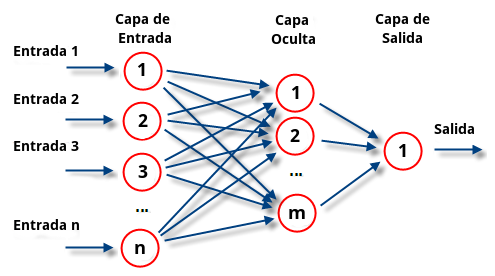
\includegraphics[width=0.8\textwidth]{img/rnn.png}
\caption{\label{fig:rnn}Red neuronal \ldots}
\end{figure}
La figura \ref{fig:rnn} muestra \ldots

\section{Introducción}
\label{sec:intro-sota}

\section{Estado del arte}
\label{sec:sota}

\section{Técnicas utilizadas}
\label{sec:tecnicas-utilizadas}

\subsection{YOLOv4 + Tensorflow 2}
\label{sec:tecnicas-utilizadas1}

\subsection{DeepSort}
\label{sec:tecnicas-utilizadas2}

\section{Conclusiones}
\label{sec:conclu-sota}

\chapter{Desarrollo algoritmo de objetos abandonados}
\label{cha:desarrollo}

\section{Introducción}
\label{sec:intro-alg-abandono}

\section{Desarrollo del algoritmo}
\label{sec:alg-abandono}


\begin{table}[!h]
\centering
\begin{tabular}{|c|c|c|c|c|}
\hline
Esto & es & una & tabla & sencilla \\ \hline
1    & 2  & 3   & 4     & 5        \\ \hline
6    & 7  & 8   & 9     & 10       \\ \hline
11   & 12 & 13  & 14    & 15       \\ \hline
\end{tabular}
\caption{Esto es una tabla ejemplo}
\label{tab:my-table}
\end{table}

\section{Conclusiones}
\label{sec:conclu-alg-abandono}

\chapter{Resultados}
\label{cha:resultados}

Aquí se mostrarán los resultados del proyecto \ldots

Como dijo \cite{einstein} \ldots

\section{Introducción}
\label{sec:intro-resultados}

\section{Entorno experimental}
\label{sec:desarrollo-resultados}

\subsection{Bases de datos utilizadas}
\label{subsec:bases-datos}

\subsection{Métricas de calidad}
\label{subsec:metricas-calidad}

\subsection{Estrategia y metodología de experimentación}
\label{subsec:estrategia-metodologia}

\section{Resultados experimentales}
\label{sec:resultados-experimentales}

\section{Conclusiones}
\label{sec:conclu-resultados}

\chapter{Conclusiones y líneas futuras}
\label{cha:concl-lineas-futuras}

En esta sección se hablará sobre futuros proyectos derivados de éste \ldots

\section{Conclusiones}
\label{sec:conclusiones-finales}

\section{Líneas futuras}
\label{sec:lineas-futuras}

% Bibliografía
\bibliography{biblio/biblio.bib}
\bibliographystyle{IEEEtran}

% Anexos
\begin{appendices}
\chapter{Pliego de condiciones}
\label{cha:pliego-de-condiciones}

\section{Introducción}

En este apartado se evaluaran las condiciones para poner en marcha el software que se ha especificado en los apartados anteriores. Cabe resaltar el carácter de este proyecto, en el que se ha diseñado una colección de funciones que facilitan al programador la correcta adquisición de datos sonoros, y por lo tanto no aplican las condiciones técnicas o ambientales que pudieran afectarle, ya que las impone los requerimientos las aplicaciones que en un futuro se le quiera dar a este proyecto.

Solamente afectan las condiciones de configuración hardware o software donde se quiera aplicar el programa informático.

\section{Requisitos de hardware}

\subsection{Requisitos mínimos}
\begin{itemize}
  \item Utilización de un PC de 32 bits de escritorio con tarjeta de sonido.
  \item Un mínimo de 384 MB de memoria RAM.
  \item Al menos 100 MB de memoria libre en disco duro.
\end{itemize}

\subsection{Requisitos de hardware recomendados}
Estos requisitos son necesarios para implementar algoritmos de localización basados en onda sonora.
\begin{itemize}
  \item CPU de 64 bits con 4 Cores o más.
  \item Sistema de adquisición con 8 canales o más.
  \item Utilización de al menos 4 Gb de memoria RAM.
\end{itemize}

\section{Condiciones hardware}

El sistema de adquisición que se propone hace uso de 4 hilos independientes en la adquisición en tiempo real. Es por esta razón que se recomienda sistemas multiprocesador, que permitan realizar las tareas de cada hilo de manera independiente.

Se precisa de un sistema de adquisición de audio profesional para la adquisición del audio proveniente de cada micrófono para ejecutar el algoritmo de localización. Además por esta razón y porque se van a generar gran cantidad de datos a procesar en la memoria RAM del equipo, es necesaria la utilización de un volumen importante de memoria RAM, se recomienda que la cifra de partida sean 4 Gb que es la cifra máxima que un sistema operativo de 32 bits basado en Linux puede direccionar.

Se recomienda tener 100 MB de disco duro libre para poder hacer grabaciones de corta duración. Es altamente recomendable disponer de 10 GB libres si se van a realizar grabaciones multicanal y de larga duración.
 
\section{Requisitos de software}

\subsection{Requisitos mínimos}
\begin{itemize}
  \item Utilización de un sistema operativo Ubuntu 12.04.
  \item Librería \texttt{Rtaudio}.
  \item Librería \texttt{SNDFile}.
  \item Para el desarrollo del algoritmo de localización se deben utilizar las librerías propias del grupo GEINTRA.
\end{itemize}

\subsection{Requisitos de software recomendados}
\begin{itemize}
  \item Utilización de un sistema operativo de 64 bits, Ubuntu 12.04 o superior.
\end{itemize}

\section{Condiciones software}

En este apartado software se recomienda utilizar el sistema operativo Ubuntu 12.04 al ser LTS, y proporcionar la compatibilidad con las nuevas librerías Qt para realizar profiling mediante KCachegrind.

En el caso de disponer un sistema hardware con una memoria RAM superior a 4 GB es necesario utilizar, una verisón de Ubuntu de 64 bits para poder direccionarla. Es muy recomendable esta opción para poder adquirir y procesar sonido multicanal.

\newpage
\section{Condiciones generales}

La utilización de esta librería supone la posibilidad de ejecutar cualquier programa de procesamiento sobre ella que tenga en cuenta las siguientes condiciones:

\begin{itemize}
  \item El ancho de banda de las señales acústicas está condicionado por el rango que permita la tarjeta de adquisición a utilizar, por lo general cumple aproximadamente la del espectro del oído humano, de 20 a 20000 Hz.
  \item El número de canales a utilizar lo limita la tarjeta de adquisición, la librería está preparada para adquirir, sea cual sea el rango multicanal.
  \item Ante cualquier uso de esta librería deberá tenerse en cuenta el reconocimiento (BY), que no es comercial (NC), y que las obras derivadas se compartan de igual manera (SA).

\end{itemize}

\chapter{Presupuesto}
\label{cha:presupuesto}

\section{Equipo de trabajo}

Para la realización del proyecto se va a necesitar un Ingeniero de Telecomunicaciones.

\section{Timing}

Las fases necesarias para la realización del desarrollo son las siguientes.

\begin{itemize}
  \item Configuración del hardware (0,5 meses)
  
  \begin{itemize}
    \item Instalación de sistema operativo, librerías, IDE. (0,25 meses)
    \item Configuración y puesta en marcha. (0,25 meses)
  \end{itemize}
  
\item Diseño e implementación de los módulos software necesarios (6 meses):
  
  \begin{itemize}
    
  \item Diseño e implementación de librerías de soporte para la
    reproducción y adquisición de audio multicanal temporizado (tiempos
    fijos) (2 mes).
    
  \item Diseño e implementación de librerías de soporte para la
    adquisición, reproducción y procesamiento de audio multicanal
    continuo (tiempo indefinido) (4 mes).
    
  \end{itemize}
  

\item Evaluación del sistema de procesamiento de audio multicanal (1,5 meses):
  
  \begin{itemize}
    
  \item Adaptación del algoritmo SRP. (0,5 meses)
  
  \item Evaluación del sistema de adquisición sobre la librería de tiempo real (1 mes)
    
    \end{itemize}
  
\item Documentación

\end{itemize}

Por supuesto, las fases de diseño, desarrollo, pruebas y documentación
son cíclicas y abarcan todo el periodo de la vida del proyecto.


\section{Presupuesto total}

Por todo lo anterior, supone una duración de 8 meses naturales con un coste de 12.000 \euro (sin IVA).


\chapter{Manual de usuario e instalación}
\label{cha:manual-usuario}

\section{Introducción}
\label{sec:intro-manual-de-usuario}

Blah, blah, blah\ldots


\section{Manual}
\label{sec:sec-manual-de-usuario}

Pues eso.


\section{Ejemplos de inclusión de fragmentos de código fuente}
\label{sec:codigo-fuente}

Ahora compila usando \texttt{gcc}:

\begin{enumerate}
\item bla bla:

\begin{lstlisting}
$ python object_tracker.py --video ./data/video/video1.avi

\end{lstlisting}

\end{enumerate}



\end{appendices}

% Contraportada

\includepdf[pages={6}]{cover/portada.pdf}

\end{document}
